\documentclass[11pt,a4j,notitlepage]{jreport}
\usepackage{TUSGradThesis}

\usepackage[dvipdfmx]{graphicx}
\usepackage[dvipdfmx]{color}
\usepackage{amsmath,amssymb}
\usepackage{setspace}
\usepackage{fancyhdr}
\usepackage{amsmath}
\usepackage{bm}
\usepackage{here}
\usepackage{multirow}
\usepackage{ascmac}
\usepackage[dvipdfmx]{color}
\usepackage{subfigure}
\usepackage{cases}
\usepackage{setspace}
\usepackage{subfiles}
\usepackage{algorithm}
\usepackage{algorithmic}
\usepackage{afterpage}
\usepackage{comment}

\makeatletter
    \renewcommand{\theequation}{%
    \thesection.\arabic{equation}}
    \@addtoreset{equation}{section}
    \def\thefigure{\thesection.\arabic{figure}}
    \@addtoreset{figure}{section}
    \renewcommand{\thetable}{%
    \thesection.\arabic{table}}
    \@addtoreset{table}{section}
\makeatother

\renewcommand\bibname{参考文献}
\newcommand{\Figref}[1]{図~\ref{#1}}
\newcommand{\Eqref}[1]{式~(\ref{#1})}
\newcommand{\Tabref}[1]{表~\ref{#1}}

\newcommand{\mymax}{\mathop{\rm max}\limits}

\makeatletter
\renewcommand{\l@figure}{\@dottedtocline{1}{1.5em}{3.2em}}
\makeatother

\makeatletter
\renewcommand{\l@table}{\@dottedtocline{1}{1.5em}{3.2em}}
\makeatother

\makeatletter
\newcommand{\subsubsubsection}{\@startsection{paragraph}{4}{\z@}%
  {1.0\Cvs \@plus.5\Cdp \@minus.2\Cdp}%
  {.1\Cvs \@plus.3\Cdp}%
  {\reset@font\normalsize\bfseries}
}
\makeatother
\setcounter{secnumdepth}{4}

\setstretch{1.5}
\setcounter{tocdepth}{2}
%\setcounter{secnumdepth}{3}

% 表紙情報
\発表年度{2021} % 全角で書くこと
\著者情報{4618023}{北田 来人}
\指導教員{藤井 孝藏 1教授,松尾 裕一 教授}{立川 智章 准教授, 浅田 健吾 助教}
\論文題目{多目的進化計算における}{設計変数の削減方法に関する研究}
{Research of reducing decision variables}{in Multi Objective Evolutionary Algorithm}

% 要旨
%\要旨{}
\begin{document}
% 表紙の出力
\titleoutput

% 要旨の出力
\gtabstract

\pagenumbering{roman}
\tableofcontents
\listoffigures
\listoftables

\clearpage
\pagenumbering{arabic}

\chapter{序論}
\section{研究背景}
近年,多目的進化計算には計算効率を悪化させる幾つかの課題が見受けられる。ここで計算効率の悪化とは、最適化の難易度が高くなり、計算コストの増加、最適化の遅延により、良い最適解を求めることが困難になることを意味する。計算効率を悪化させる幾つかの課題として、(1)目的関数の数が増大することで目的関数空間が指数関数的に大きくなること、(2)多数の制約条件や、厳しい制約条件(強制約と呼ばれる場合もある)を満足できないこと、(3)設計変数の数が某大になることで「次元の呪い」と言われる事象が発生することが挙げられる(「次元の呪い」については後ほど説明する)。1つ目と2つ目の課題に関しては目的関数や制約条件の評価方法を工夫することにより、多数目的かつ強制約問題の最適化に対応でき始めている。しかし、3つ目の課題、設計変数の数が膨大な場合においては未だ不十分であり、計算効率の悪化が著しい。
\\
進化計算は数値最適化、組合せ最適化、制約最適化など様々な場面で利用されている。それに伴い実問題においても進化計算が利用され、限られた計算回数で、設計変数の数が莫大な多目的最適化問題を解くことは強く求められている。例えば,車体設計情報抽出に適した多目的可視化に関する研究1)では車体の部品を設計変数として用いる際に、200以上の設計変数が使用された。また、空気力学の形状最適化問題での設計変数は何千もあると記載3)されている。研究背景として留意していただきたいことは、設計変数が莫大になること(設計変数の次元数が莫大になること)による計算効率の悪化は「次元の呪い」4)と呼ばれる。次元の呪いと呼ばれるには二つの理由がある。\\一つ目に実行可能領域は、次元数の増加に伴い指数関数的に大きくなる一方で、限られた時間で有望な実行可能領域をより効率的に探索する戦略が求められるようになっていること。\\二つ目に次元数の増大は問題の特徴を変えうること。例えばローゼンブロック関数が2次元では単峰性であるのに対して、それ以上の次元では多峰性に変わるように設計変数の数すなわち設計変数の次元数が異なることで問題の特徴が変わるのである4)。\\以上の2つは設計変数が増大することにより引き起こされ、これらの事象を対処する最適化戦略はもはやないとまで言われており、目下盛んに研究が行われている。

\section{研究目的}
本研究では膨大な数の設計変数を主成分分析を用いてグルーピンを行い、グルーピングを行った複数の解を良い解を求められる方向にまとめて進化させ、膨大な設計変数すなわち高次元の設計変数空間をもつ多目的最適化問題を低次元のものへと擬似的に表し、効率的に解くことを目的とする。
\section{本論文の構成}
本論文は「多目的進化計算における設計変数の削減方法に関する研究」と題し,
5 章より構成されている.
\\
第 1 章
「序論」では,本研究を取り組むにあたっての背景と本研究の目的を明らかにし、説明を行う。

第 2 章
「多目的進化計算」では,本研究で取り扱う多目的最適化について論じる.多目的最適化問題及び,多目的最適化における進化計算,遺伝的アルゴリズムなど,本研究に関わる内容を中心にまとめる.

第 3 章
「研究方法」
第 4 章
「結果と考察」第 3 章で示した

第 5 章
「結論」
今後の課題と展望について論じる.
\chapter{多目的進化計算}
はじめに, 本章では多目的最適化進化計算に関して説明を行う。2.1節では, まず多目的最適化問題について, また多目的最適化で重要な概念となるパレート最適解について説明する.
2.2節では, 3種類の多目的進化計算について説明する.
2.3節では, 本研究で利用される主成分分析について説明する.
\section{多目的最適化問題}
\subsection{最適化}
最適化(optimization)とは,何らかの価値基準に対して最も適した解を見つけることである.工学設計ではこのような価値基準として,コスト,製品の性能,重量などの様々な問題に応じて各々基準が取られる.通常は次のような数理計画として定式化(MP)とされる
\begin{eqnarray}
(MP)         \mbox{目的}&:& f(x)\mbox{ → }min\\
         \mbox{制約}&:&x    \in  X.
\end{eqnarray}
ここで$x$は設計変数,$f(x)$は目的関数と呼ぶ.しかし,問題によっては最大化を求められる場合もあるがその時は$-f(x)$の最小化問題と捉えれば良い1.

\subsection{多目的最適化問題}
実世界の最適化問題の多くは,複数の目的が内在する多目的最適化問題(multi-objective optimization)である.自動車の設計では,「車体性能の最大化と車体部品数の最小化」を追求することに例えられる.車体性能の最大化を追求すれば,部品数は増やさざるを得ない.部品数の最小化を追求すれば,車体性能は落とさざるを得ない.このような,実世界の最適化問題で考慮する複数の目的は,相反の関係になることが多い.そのため,多目的最適化問題では,すべての目的に最適な唯一の最適解は存在しない.そのような場合に複数の目的に関して最適化を行いたい場合に多目的最適化が扱われ,与えられた設計変数と制約条件において,複数の目的関数に対して最小化(最大化)する問題を多目的最適化問題と呼び,一般に次のように定式化される.x
\begin{eqnarray}
(MOP)         \mbox{目的}&:& f(x):=(f_1(x),f_2(x),..............,f_n(x))\mbox{ → }min\\
         \mbox{制約}&:&x    \in  X.
\end{eqnarray}
 
\subsection{パレート最適解}
ある目的関数値に注目すると優れている解でも他の目的関数値においては劣っているような解が存在する。このようなトレードオフ関係にある多目的最適解をパレート最適解と呼ぶ.パレート解は唯一に定まらず,比較して優越がつけられない2つ以上の解が存在するはずであり、全てのパレート解を要素にもつ集合のことをパレートフロントと呼ぶ.多目的最適化問題の解兄おける優越関係は以下のように定義されている。多目的最適化問題における解の優越関係の定義を以下に示す.ここでは, 全ての目的が最小化問題と仮定した場合のみ示す.
\begin{eqnarray}
        f_i(x) &\leq & f_i(y)    \hspace{10mm}  \forall i \in \{1,2,3,.....,N\} \\
        f_i(x) & < & f_i(y)       \hspace{10mm} \forall i \in \{1,2,3,.....,N\} \\
        x,y &=& (x_1,x_2,....,x_n)
\end{eqnarray}
式(2.1.5)では, $x$が$y$に優越するという.
式(2.1.6)では, $x$が$y$に強い意味で優越するという.
この場合, $x$は$y$よりも良い解であることを意味する.
ある解を対象として, $f(x) \leq f(\hat{x})$となるような$x \in X$が存在しないとき,この$\hat{x}$をパレート最適解という。$f(x) < f(\hat{x})$となる$x \in X$が一つでも存在しない場合,その解を弱パレート最適解と呼び, 優越する解が存在しない場合, パレート最適解と呼ぶ.
\section{多目的進化計算手法}
進化計算とは,進化論、遺伝学、遺伝子工学の知識を融合し、生物の進化をコンピュータ上で模倣したものが、進化的アルゴリズム、別名進化的計算,進化計算である。多目的最適化問題では,各目的関数がトレードオフ関係にある場合,一つの最適解を求めることは難しいため、パレート最適解の集合が求められることが望ましい.そこで,進化的計算は複数の個体が一斉に解を探す個体群ベースアプローチ (population-based approach) のため、複数の解を探す多目的最適化には非常に好都合な手法である.
進化計算の基本的なフローチャートは図2.2.1に示し。流れを以下に説明する。

\begin{itembox}[l]{進化計算の流れ}
\begin{enumerate}
  \item 最初に乱数で個体群を生成する。ここで良い解を生成できれば最適化がよりよく働く
  \item 個体群が環境に適しているかどうかの評価をする。例えば扱う多目的最適化問題が全て最小化問題ならば、個体群の中で全ての関数値が小さいものから良い解と評価して優劣をつける
  \item 2.で評価した個体群から必要な数の個体を選択し、親個体群を生成する
  \item 親個体群から遺伝的オペレータと呼ばれる交叉や突然変異などの操作により子個体群を生成する
  \item 生成した子個体群に対して環境に適しているかどうかの評価をする
  \item 計算は事前に与えられた条件(世代数や関数評価回数)を満たすと終了する.満たしていない場合、環境適合の度合いに応じて選択・淘汰を行う.選ばれた個体は次世代の親個体となり、4へ戻り同様の流れを繰り返すことによって環境に適した個体に進化していく。
\end{enumerate}
\end{itembox}

\begin{figure}[htbp]
	\begin{center}
		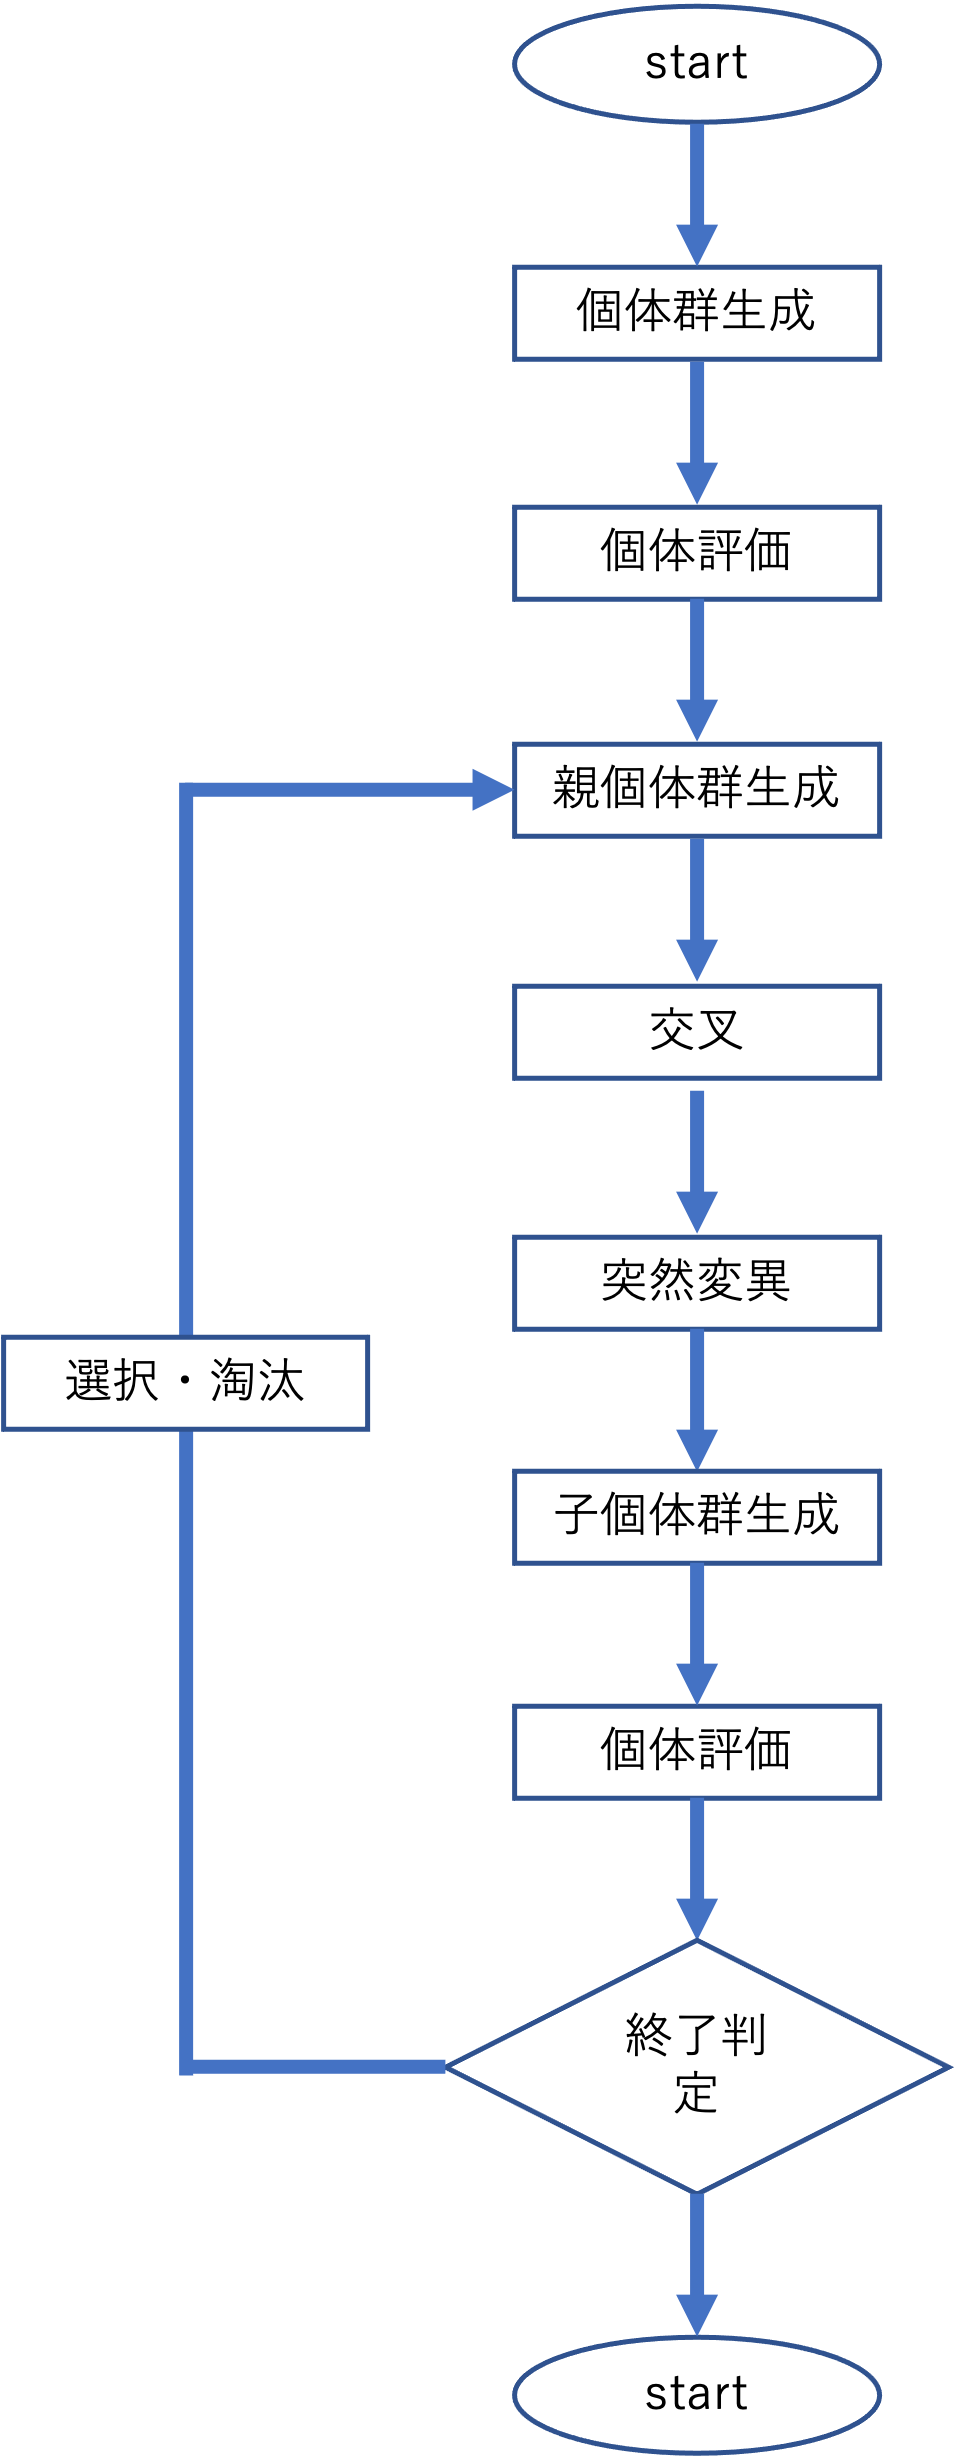
\includegraphics[width=0.55\linewidth]{fig2.png}
             		\setlength{\abovecaptionskip}{0mm}
		\setlength{\belowcaptionskip}{0mm}
			\caption{進化計算の基本的な流れ}
	\label{fig:GA}
	\end{center}
\end{figure}
\newpage

\subsection{Non-dominated Sorting Genetic Algorithms-II : NSGA-II}
NSGA-II\cite{Deb}はSrinvasとDebらが提案したNon-dominated Sorting Genetic Algorithm(NSGA)に生存選択法としてエリート主義を導入したアルゴリズムであり, Debらによって提案された.
NSGA-IIは収束性の評価軸にパレートランキング法を, 多様性の評価軸として混雑距離と混雑比較オペレータを導入している.
パレートランキング法の概念図を図 \ref{fig:ranking}に示す.

\begin{figure}[htbp]
  \begin{center}
  \subfigure[Rank1の計算]{
    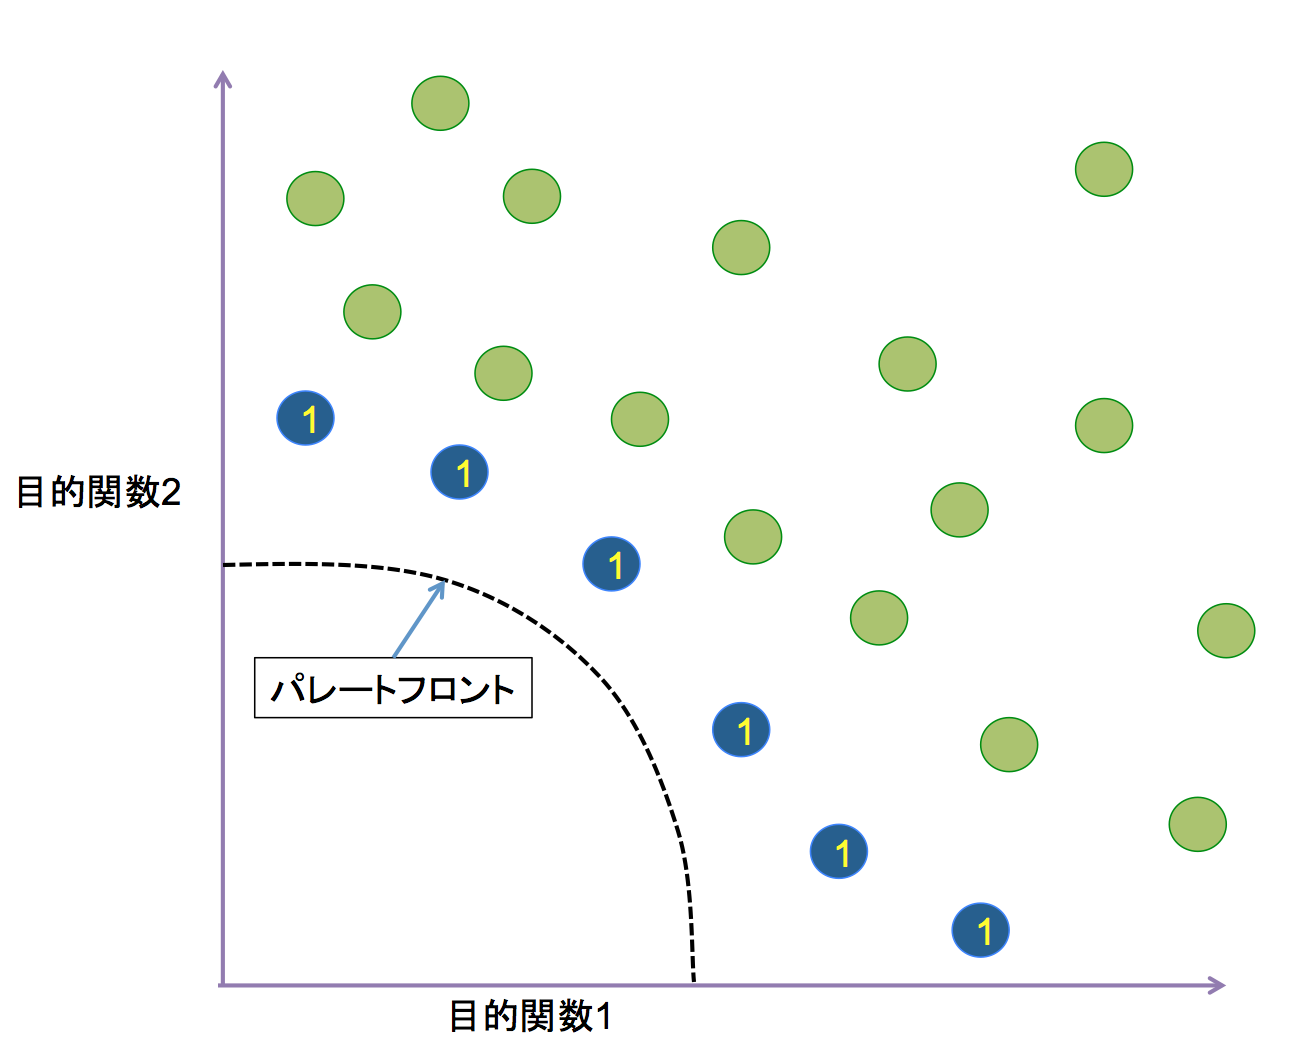
\includegraphics[width=0.3\linewidth]{img/Rank1.png}
    \label{fig:dtlz3_credit1}
    }
     \subfigure[Rank2の計算]{
    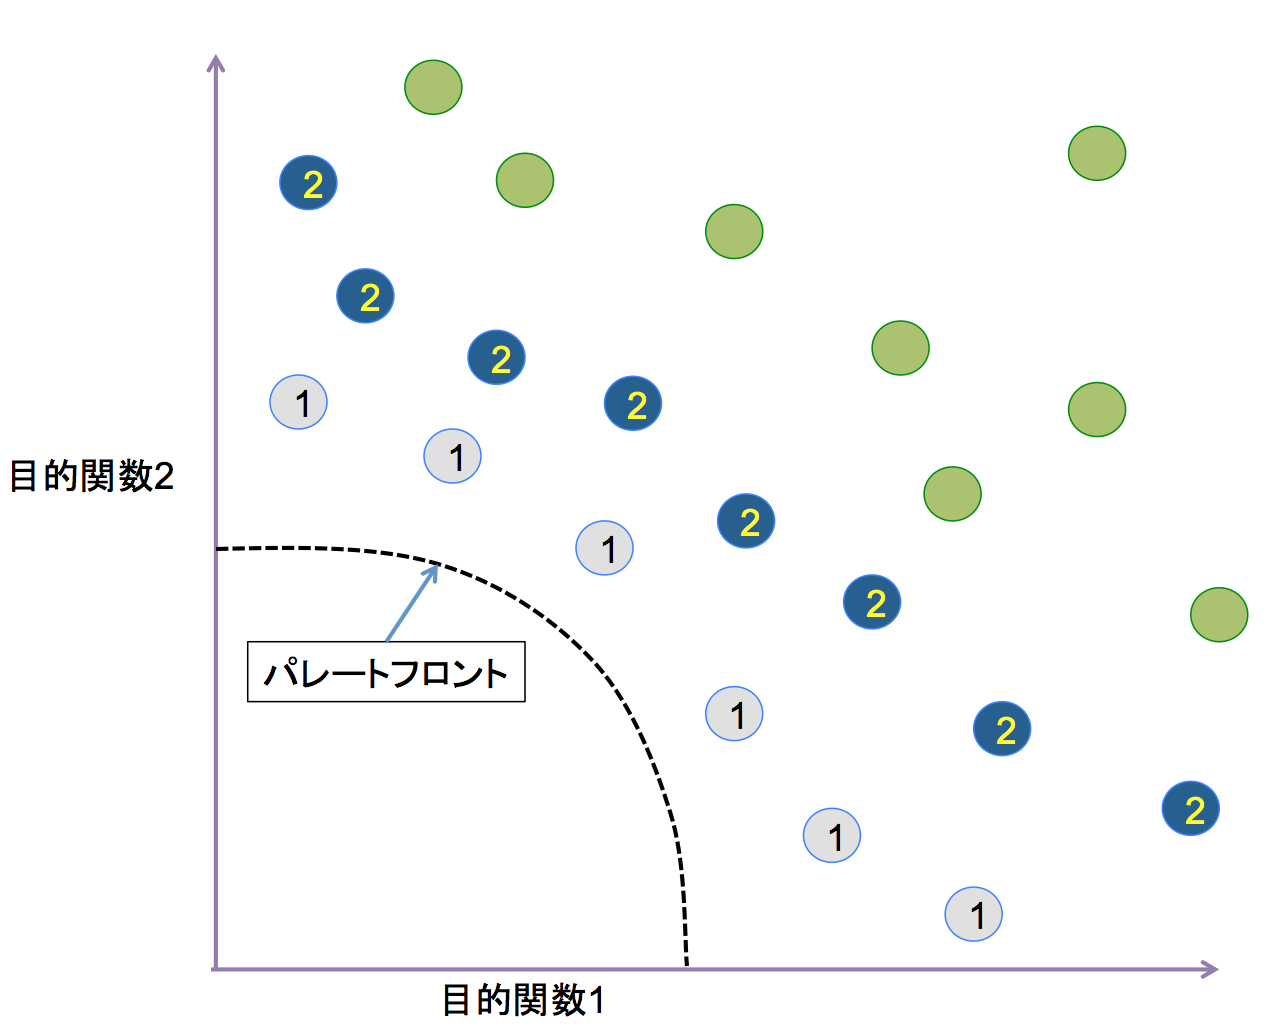
\includegraphics[width=0.3\linewidth]{img/Rank2.png}
    \label{fig:dtlz3_credit2}
    }
    \subfigure[Rank5の計算]{
    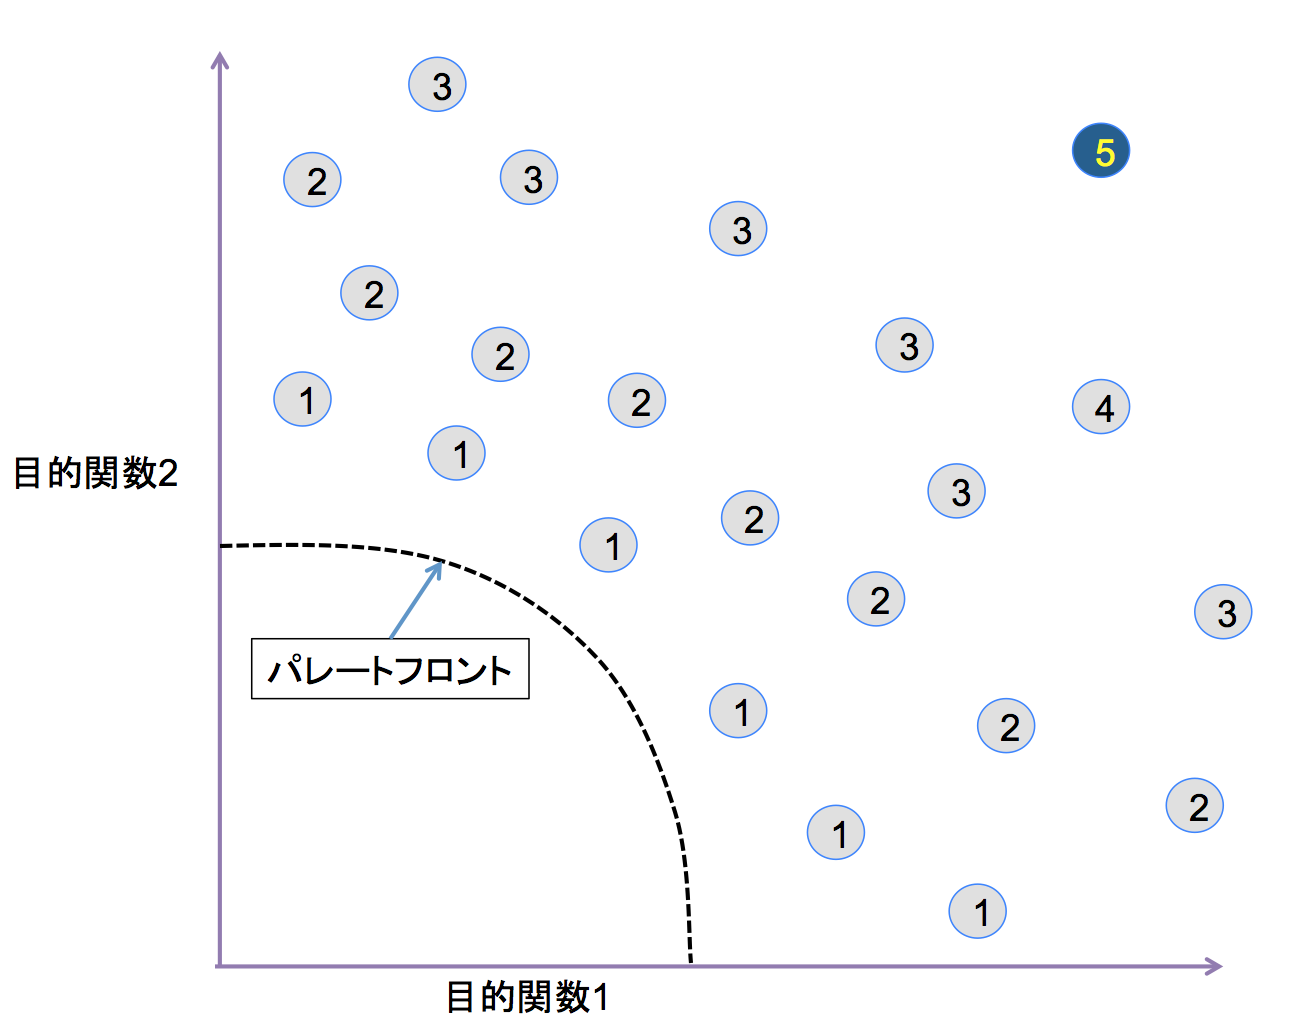
\includegraphics[width=0.3\linewidth]{img/Rank5.png}
    \label{fig:dtlz3_credit1_improve}
    }

                \setlength{\abovecaptionskip}{0mm}
    \setlength{\belowcaptionskip}{0mm}
      \caption{パレートランキング法}
  \label{fig:ranking}
  \end{center}
\end{figure}

\vspace{3mm}
パレートランキング法では, 集合の中で他のどの個体にも支配されない解をRank1とする.
次に, Rank1の解を除いた集合の中で他のどの個体にも支配されない解をRank2とする.
この繰り返しを全個体でRankが決まるまで行う.
図\ref{fig:ranking}では, 最大Rankは5となる.
また, NSGA-IIではこのランキングの高速化した高速優越ソートを用いている.
高速優越ソートの手順を以下に示す.


\begin{enumerate}
\item 各個体に対して, 支配している個体の数と支配されている個体の数を同時に計算する.
\item Rank1の個体のみをリスト1にまとめる.
\item リストF$_1$に含まれる各個体が支配している個体に対して, 支配されている数を1ずつ引く.
\item 上記同様, Rank1(支配されている数が0)の個体のみをリストF$_2$にまとめる.
\item 1 $\sim$ 4を全個体が無くなるまで繰り返す.
\end{enumerate}

次に, 混雑距離について説明する.
混雑距離の概念図を図 \ref{fig:crowd}に示す.

\begin{figure}[htbp]
  \begin{center}
    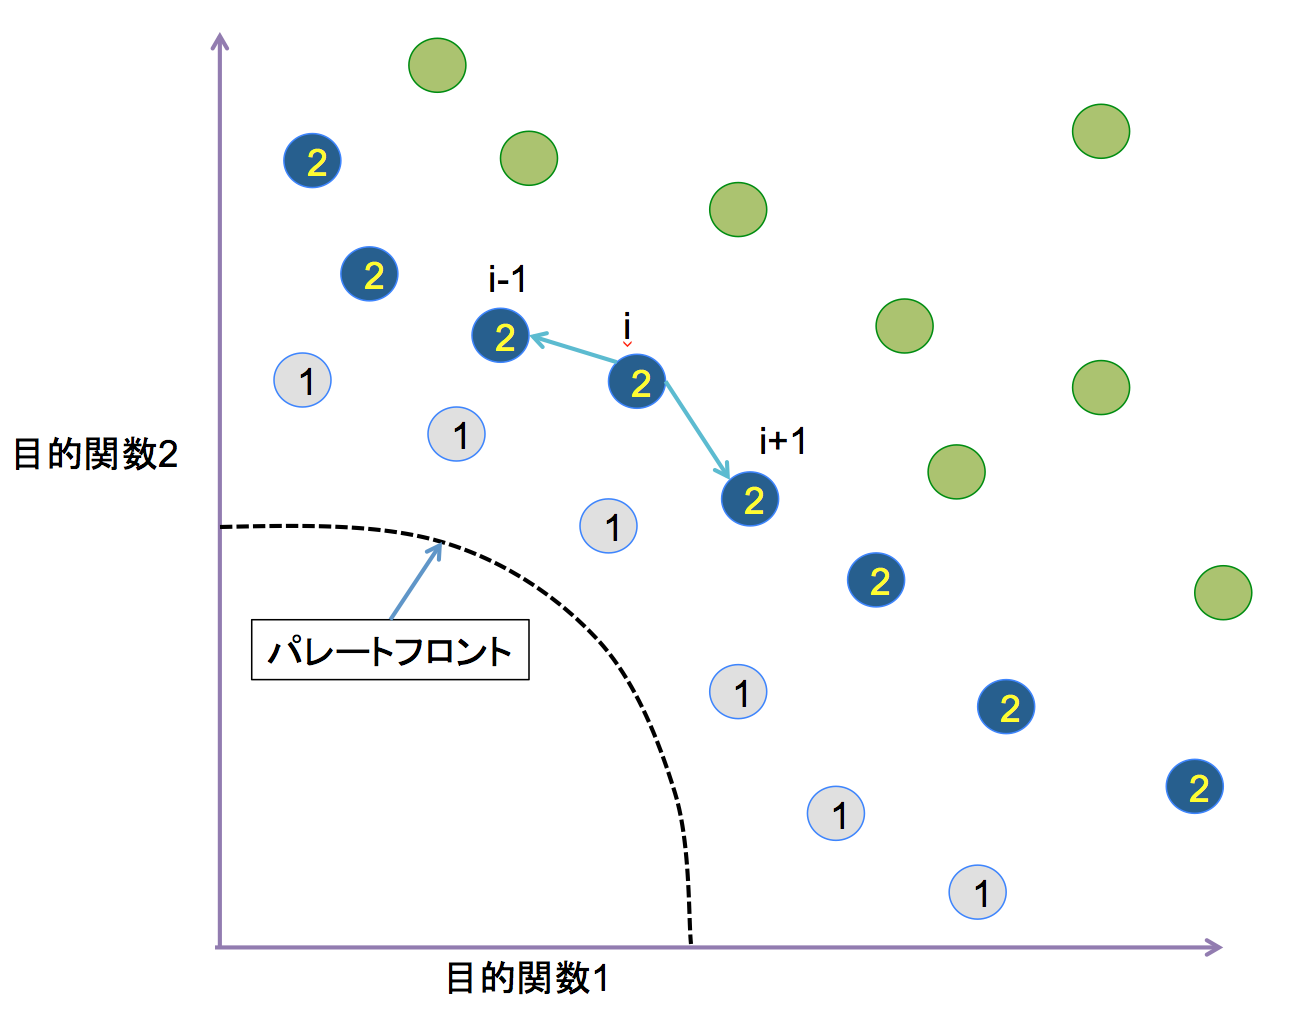
\includegraphics[width=0.7\linewidth]{img/Crowd.png}
                \setlength{\abovecaptionskip}{0mm}
    \setlength{\belowcaptionskip}{0mm}
      \caption{混雑距離の計算法}
  \label{fig:crowd}
  \end{center}
\end{figure}


混雑距離は, 同一ランク内の集団を目的関数値でソートし, 両隣に隣接する個体との距離の和を計算する.
この計算は全個体で行われ, 各目的関数において端に位置する個体は無限大が割り振られる.

最後にNSGA-IIで用いられるエリート主義について説明する.
NSGA-IIのエリート主義の概念図を図 \ref{fig:nsgaii}に示す.
\begin{figure}[htbp]
  \begin{center}
    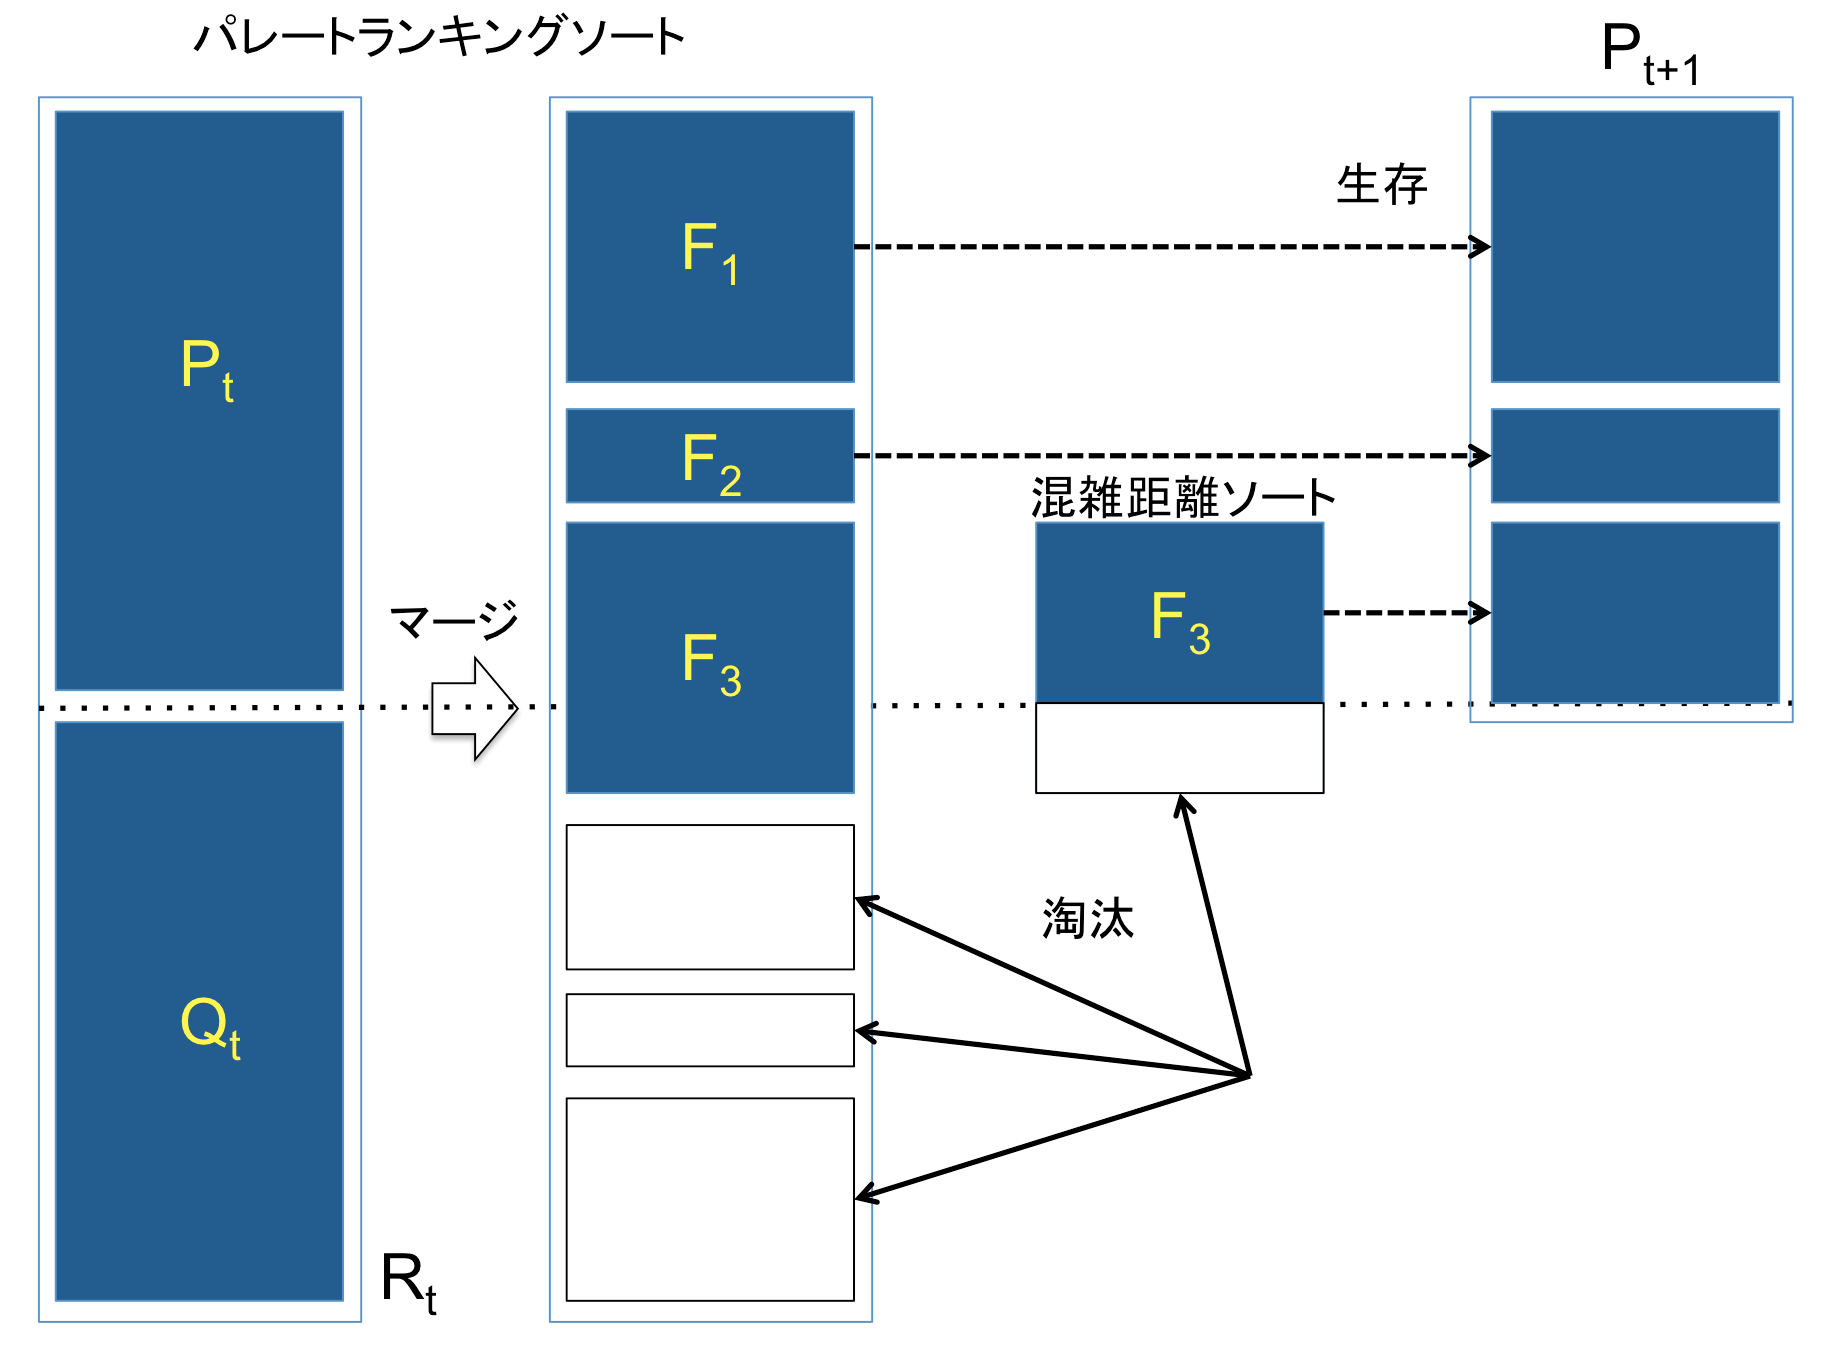
\includegraphics[width=0.7\linewidth]{img/NSGAII.png}
                \setlength{\abovecaptionskip}{0mm}
    \setlength{\belowcaptionskip}{0mm}
      \caption{NSGA-IIのエリート主義の概念図}
  \label{fig:nsgaii}
  \end{center}
\end{figure}

N個の個体で計算を行う場合, 毎世代N個の親個体P$_t$と, P$_t$から交叉, 突然変異によって新しく生成されるN個の子個体Q$_t$の合計2Nの個体が得られる.
2N個の個体から次の世代に使用するN個の親個体P$_{t+1}$の選択にエリート主義が使用される.
まずP$_t$とQ$_t$をマージした上で, パレートランキングによって各個体のランクを計算し, ランク順にソートを行う.
Rank1から順に, 合計数がNを超えないランクまでP$_{t+1}$に追加する.
P$_{t+1}$の個体数がNを超えてしまうランクでは, そのランク内の全個体で混雑距離を計算し, 値が大きい順にソートする.
そこで, P$_{t+1}$の個体数がNになるまで混雑距離のソートした順番に追加する.
端に位置する個体は混雑距離の値が無限大になるため, 必ず選択されるようになっている.

\subsection{Non-dominated Sorting Genetic Algorithms-III : NSGA-III}

NSGA-III\cite{Jain}は,Debらにより提案され,目的数が4以上の多目的最適化問題において,高い探索能力となるようNSGA-IIを改良した探索手法である.
NSGA-IIとの大きな違いは,多様性維持のための機構が異なっている点である.NSGA-IIIでは, reference lineに基づく個体選択により探索を行っている.

refenrence line および reference pointの概念を説明する.
初めに評価値空間上に均等に reference point を配置する. reference pointは,目的数を $M$ ,分割数を $p$ とすると
\[
  A = \left(
    \begin{array}{cc}
      M + p - 1 \\
            p
    \end{array}
  \right)
\]
個生成される. reference point の目的数が 3 ,分割数が 4 の例を\ref{fig:nsgaiii}に示す.
\begin{figure}[htbp]
\begin{center}
  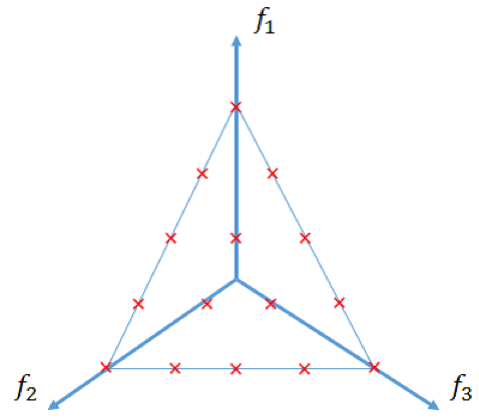
\includegraphics[width=0.7\linewidth]{img/NSGAIII.png}
                \setlength{\abovecaptionskip}{0mm}
  \setlength{\belowcaptionskip}{0mm}
    \caption{reference point の配置(M = 3 , p = 4)}
\label{fig:nsgaiii}
\end{center}
\end{figure}

reference lineとは,各 reference point と原点を通る線のことを表す.主な演算の流れはNSGA-IIと類似している.
NSGA-IIでは解の優越関係と混雑距離に基づいたエリート選択によって次世代個体の選択を行うが,
NSGA-IIIの次世代個体の選択では,次世代個体群の数が設定された個体数を超えない間は,NSGA-IIと同様に,ランクの高い個体から順に次世代個体に選択する.
探索個体数を超える場合には,混雑距離に代わり, reference line に基づいた選択により次世代に残す個体を決定する.以下に, reference line を用いた次世代個体の選択方法を説明する.

まず,個体 P$_i$ について,評価値空間上での距離が最も近い reference line L$_j$ を,個体 P$_i$に対する近傍ラインと定義する.また,L$_j$を近傍ラインとする個体を L$_j$に対する近傍個体と定義する.

\begin{enumerate}
\item すでに次世代個体に選択されている個体に対し,それぞれ近傍ラインを割り振る.
\item 近傍個体数の最も少ない reference line を選び,対象ランクの個体群のうち,その reference line の近傍個体の中から最も距離の近い個体を次世代個体群に加える.
\item 次世代個体群の数が設定された個体数を満たすまで 2 を繰り返す.
\end{enumerate}

reference line を用いることにより,目的関数の数が大きい最適化問題においても,高い収束性を有することが示されている.\cite{Jain}

\subsection{MOEA/D}
\quad MOEA/D (Multi-objective Evolutionary Algorithm Based on Decomposition)\cite{Zhang2007MOEAD}は2007年にZhangらによって提案されたRCGAの一つである.
本研究においても,数値実験に使用している.

MOEA/Dでは探索空間上に重みベクトルを均一の間隔で分布させ,それらの重みベクトルとスカラー適応度関数を用いて,多目的最適化問題をベクトル毎の単一目的最適化の部分問題へと帰着させる.
その後,各重みベクトルに対し,ユークリッド距離の近いベクトルを近傍とし,近傍内において遺伝的操作(交叉や突然変異)を行う.
また,MOEA/Dでは最適化に用いる個体群とは別に,計算中に得られた非劣解群をアーカイブとして保持する機構を持つ.

MOEA/Dの計算の流れを以下に示す.

\begin{description}
\item[Step 1 : 初期化]\mbox{}\\
\vspace{-0.5in}
	\begin{description}
	\item[1.1 : 重みベクトル生成]\mbox{}\\
	探索に用いる$N$個の重みベクトル${\bm \lambda}$を\Eqref{omomi}により生成する.
	\begin{eqnarray}
	\left.
	\begin{array}{rcl}
	{\bm \lambda} & = & (\lambda_1, \lambda_2, \cdots, \lambda_k)\\
	\sum_{i=1}^{k} \lambda_i & = & 1\\
	N & = & {}_{H+k-1}C_{k-1}\\
	where & \lambda_i & \in \left\{ \cfrac{0}{H}, \cfrac{1}{H}, \cdots, \cfrac{H}{H} \right\}
	\end{array}
	\right\}
	\label{omomi}
	\end{eqnarray}

	ここで,$k$は目的関数の数,$H$は分割数を表す.

%	\vspace{-0.1in}

	\item[1.2 : 近傍ベクトル生成]\mbox{}\\
	1.1で作成した各ベクトル間のユークリッド距離を計算し,各ベクトル$\bm \lambda^i$に最も近い$T$個のベクトル$\bm \lambda^{i_1}, \cdots, \bm \lambda^{i_T}$を$\lambda^i$の近傍とする.
%	\vspace{-0.1in}

	\item[1.3 : 初期個体群生成]\mbox{}\\
	ベクトルの総数$N$個と等しい数の初期個体をランダムに生成し,1つのベクトルに対し1つの個体を対応させる.
%	\vspace{-0.1in}

	\item[1.4 : 参照点更新]\mbox{}\\
	参照点$\bm z^*$の更新を\Eqref{sansyou}によって行う.

	\begin{eqnarray}
	\left.
	\begin{array}{rcl}
	{\bm z^*} & = & (z_1^*, z_2^*, \cdots, z_k^*)\\
	z^*_j & = & \max \left\{ f_j (\bm x) | \bm x \in \bm X \right\}
	\end{array}
	\right\}
	\label{sansyou}
	\end{eqnarray}

	ここで,$f_j (\bm x)$は個体$\bm x$の$j$番目の目的関数,$\bm X$は設計変数空間内での実行可能領域を表す.

	\vspace{-0.1in}

	\end{description}
\item[Step 2 : 遺伝的操作]\mbox{}\\
\vspace{-0.5in}
	\begin{description}
	\item[2.1 : 親個体選択]\mbox{}\\
	ベクトル$\bm \lambda^i$の近傍ないからランダムに2つの個体を選択する.
%	\vspace{-0.1in}

	\item[2.2 : 子個体生成]\mbox{}\\
	2.1で選択された親個体から交叉(SBX)と突然変異(polynomial mutation)を行い子個体を生成する.
%	\vspace{-0.1in}

	\item[2.3 : 参照点更新]\mbox{}\\
	\Eqref{sansyou}を用いて参照点を更新する.
%	\vspace{-0.1in}

	\item[2.4 : 近傍解更新]\mbox{}\\
	2.2で生成された子個体と$\bm \lambda^i$近傍内のベクトルに対応する個体をスカラー適応度関数を用いて比較し更新する.
	スカラー適応度関数は主に Tchebycheff Approach と Weighted Sum Approach がある.
	本研究で用いるTchecycheff Approach を以下に示す.

	\begin{eqnarray}
	\left.
	\begin{array}{rccl}
	minimize & g^{te} (\bm x|\bm \lambda , \bm z^*)& =& \mymax_{1 \leq i \leq m} \{ \lambda_i|f_i (\bm x) - z^*_i| \}\\
	sub.to & x \in X &  &  \\
	where & z^* & = & (z_1^*, \cdots, z^*_k)^T
	\end{array}
	\right\}
	\label{sansyou}
	\end{eqnarray}


%	\vspace{-0.1in}

	\item[2.5 : アーカイブ更新]\mbox{}\\
	非劣解となった子個体をアーカイブに追加し,アーカイブ内の劣解を削除する.
	\vspace{-0.1in}

	\end{description}
\item[Step 3 : 終了判定]\mbox{}\\
%\vspace{-0.5in}

\end{description}


上述のアルゴリズムにおいて,Step2の操作を終了判定を満たすまで繰り返すことで解の探索を行う.


\section{解の評価指標について}
\quad 本項では,本研究で用いた多目的最適化における解の評価指標について述べる.

\subsection{GD}
Generational Distance (GD)\cite{Deb2002Fast} とは解の収束性を評価する際に用いる評価指標である.
GDは,得られた非劣解集合の各点から真のパレートフロントまでの最短距離の平均値を算出する指標である.
値が小さいほど収束性が良いことを示し,0が最小値となる.
GDは\Eqref{gd_formulation}で定式化される.

\begin{eqnarray}
\begin{array}{rcl}
GD(\bm S,\bm P)&=&\cfrac{\left( \sum^{|\bm S|}_{i=1} d_i^2 \right) ^ {1/2}}{|\bm S|}\\
d_i & = & \min_{\vec p \in \bm P} || F(\vec{s_i}) - F(\vec p) ||
\label{gd_formulation}
\end{array}
\end{eqnarray}

$\bm S$は得られた非劣解集合,$\bm P$は理論上のパレートフロントの点集合を示す.
また,$d_i$は$\bm S$の各点から$\bm P$の最短距離となる点への距離を示し,$|\bm S|$は$S$の点数を示す.


\subsection{IGD}
Inverted Generational Distance (IGD)\cite{Zhou2006combining} とは解の収束性と解の多様性を同時に評価できる総合評価指標である.
IGDは,真のパレートフロントの各点から得られた非劣解集合までの最短距離の平均値を算出する指標である.
値が小さいほど収束性と多様性が良いことを示し,0が最小値となる.
IGDは\Eqref{igd_formulation}で定式化される.

\begin{eqnarray}
\begin{array}{rcl}
IGD(\bm P,\bm S)&=&\cfrac{\left( \sum^{|\bm P|}_{i=1} d_i^2 \right) ^ {1/2}}{|\bm P|}\\
d_i & = & \min_{\vec s \in \bm S} || F(\vec{p_i}) - F(\vec s) ||
\label{igd_formulation}
\end{array}
\end{eqnarray}

$\bm S$は得られた非劣解集合,$\bm P$は理論上のパレートフロントの点集合を示す.
また,$d_i$は$\bm P$の各点から$\bm S$の最短距離となる点への距離を示し,$|\bm P|$は$P$の点数を示す.





\subsection{HV}
Hypervolume(HV)は任意の参照点$W$を用いて, 得られたパレート最適解集合の各点に対してhypercube $v_i$を生成し, $v_i$の和集合の領域が占める面積, 体積を計算する.
参照点は最適化方向とは反対方向に用意することが多く, 値が大きいほどその解集合が収束性と多様性に関して優れていることを意味する.
HVは次式で定式化される.
\begin{equation}
HV(S,W)=volume(\cup_{i=1}^{|S|} v_i) \label{eq:hv}
\end{equation}
ここで$S$は最適化によって得られたパレート最適解集合, $W$は参照点を示し, $v_i$は各hypercubeを示す.
HVの計算の概念図を図 \ref{fig:hvimg}に示す.
\begin{figure}[htbp]
  \begin{center}
    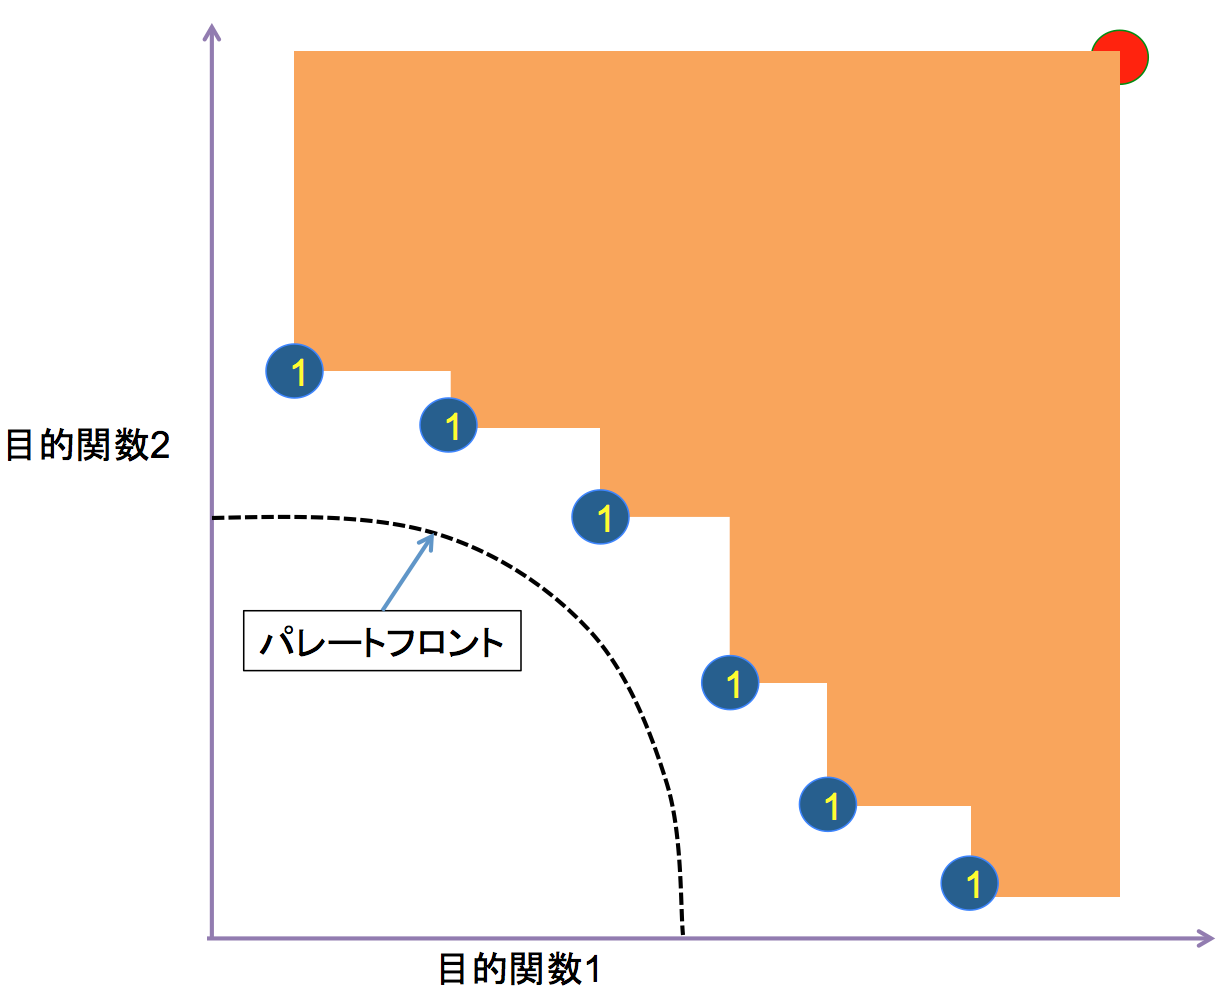
\includegraphics[width=0.7\linewidth]{img/HVimg.png}
                \setlength{\abovecaptionskip}{0mm}
    \setlength{\belowcaptionskip}{0mm}
      \caption{HVの計算の概念図}
  \label{fig:hvimg}
  \end{center}
\end{figure}

図 \ref{fig:hvimg}は2目的における概念図であり, この場合総面積がHVの値となる.
HVでは, パレートフロントが既知ではない問題でも使用できるという強みがあるが, 目的数増加および個体数の増加に伴い,計算量が急激に増加し計算が困難になる.
\section{主成分分析:Principal Component Analysis}
主成分分析とは元の情報(質的変数などの定量化できないデータで量的変数である必要がある)減らさずに次元を減らす方法である。P次元の観測変数$X=(x_1,x_2,\cdots ,x_n)$
を
\begin{thebibliography}{99}
\vspace{-1.0zh}
\bibitem{多田}多田 春樹,藤井 孝藏,立川 智章,."車体設計情報抽出に適した多目的可視化に関する研究"
\vspace{-1.0zh}
\bibitem{鐘睿}鐘 睿,高木 英行."大規模最適化問題へのスパースモデリング導入"
\vspace{-1.0zh}
\bibitem{Chai}Chai T, Jin Y, Sendhoff B,"Evolutionary complex
engineering optimization" Opportunities and challenges. IEEE Computational Intelligence Magazine
2013, 8(3):12-15.
\vspace{-1.0zh}
\bibitem{Ke}Ke Tang , Xiaodong Li , P. N. Suganthan , Zhenyu Yang , and Thomas Weise."Benchmark Functions for the CEC’2010 Special Session and Competition on Large-Scale Global Optimization"
\bibitem{Deb}K. Deb,A. Pratap,S. Agarwal,T. Meyarivan"A fast and elitist multiobjective genetic algorithm: NSGA-II"

\end{thebibliography}

\end{document}
